% !TeX encoding = utf8
% !TeX program = xelatex
% !BIB program = bibtex
% -*- coding:utf-8 mod:LaTeX -*-

% Paper 3 REVISION: Open-Set SC-BSS — cautionary / negative-result study.
% The original manuscript (main_v1_rejected.tex) claimed SNR-conditioned
% complementarity of OOD scorers and a 0.625 SNR-routed AUROC; on
% 2026-09-21 this was shown to be a repeat-vs-tile per-source SNR
% labeling artifact (see paper3_open_set/EXPERIMENT_LOG.md).  This
% manuscript is the pivot: pitfall analysis + corrected protocol +
% systematic negative result.
% Template: elsarticle (review format) — target venue: Physical Communication (Elsevier)

\documentclass[review,12pt]{elsarticle}

\usepackage{graphicx}
\usepackage{booktabs}
\usepackage{amsmath,amssymb}
\usepackage{url}
\usepackage{xcolor}
\usepackage[mode=text]{siunitx}
\sisetup{locale=US}

\usepackage{hyperref}
\hypersetup{hidelinks,
  colorlinks=true,
  allcolors=black,
  pdfstartview=Fit,
  breaklinks=true}

\usepackage{lineno}
\modulolinenumbers[5]

\usepackage{float}

\emergencystretch=1.5em

\newcommand{\snr}{\mathrm{SNR}}

\journal{Physical Communication}

\begin{document}

\begin{frontmatter}

\title{Open-Set Single-Channel Blind Source Separation:\\A Per-Source SNR-Labeling Pitfall, a Deployment-Faithful Evaluation Protocol, and a Systematic Negative Result}

\author[1]{Bin Nong\corref{cor1}}
\ead{nongbin@tfswufe.edu.cn}
\author[2]{Weihong Fu}
\author[3]{Zhuoyun Jiang}

\affiliation[1]{organization={Tianfu College of Southwestern University of Finance and Economics}, city={Mianyang}, state={Sichuan}, postcode={621000}, country={China}}
\affiliation[2]{organization={School of Telecommunications Engineering, Xidian University}, city={Xi'an}, state={Shaanxi}, postcode={710071}, country={China}}
\affiliation[3]{organization={School of Health Science and Engineering, University of Shanghai for Science and Technology}, city={Shanghai}, postcode={200093}, country={China}}

\cortext[cor1]{Corresponding author.}

% ======================================================================
\begin{abstract}
Single-channel blind source separation (SC-BSS) of co-frequency
communication signals is increasingly combined with per-source
modulation identification, and a deployed receiver must additionally
\emph{reject} sources whose modulation it has never seen. Evaluating
such open-set capability almost invariably involves conditioning
detection metrics on the operating SNR\@. We show that this conditioning
is fragile: a subtle per-source labeling convention---storing per-source
SNR labels interleaved (\texttt{np.repeat}) while the corresponding
score arrays are stacked slot-wise (\texttt{np.tile})---misaligns every
known-pool score with the wrong SNR bin and thereby \emph{manufactures}
a compelling but entirely spurious phenomenon: two out-of-distribution
(OOD) scorer families appear strongly complementary across SNR, a
training-free SNR-routed ensemble appears to lift the weighted-average
AUROC from 0.50 to 0.625, and the effect appears multi-seed significant,
robust to SIR/timing/carrier-offset perturbations, and gracefully
degrading under SNR-estimation error. Every one of these properties is
an artifact of the misalignment. We dissect the mechanism, explain why
it survives exactly the checks practitioners trust, and show how it was
caught---by sample-level alignment verification required to deploy a
real blind SNR estimator. We then re-run the entire study under a
corrected, deployment-faithful protocol (strict train/reference/test
separation, unknown-free threshold calibration, verified labels) across
six post-hoc OOD scorers, five seeds, SIR/timing/CFO perturbations,
center-loss and embedding-dimension interventions, carrier-frequency
separations, leave-one-modulation-out splits, a second attention-free
backbone, and single-threshold operating points. The corrected
finding is a systematic \emph{negative} result: per-source detection of
unknown modulations from separation embeddings is at chance everywhere
(routed $0.498 \pm 0.020$; six-scorer oracle ceiling $0.549 \pm 0.031$;
unknown detection rate $0.058$ at a calibrated 5\% false-rejection
operating point). We attribute this to the separation objective, which
shapes no known/unknown margin, and distill a protocol checklist for
future open-set evaluations in signal processing.
\end{abstract}

\begin{keyword}
Blind source separation \sep Co-frequency communication \sep Open-set
recognition \sep Out-of-distribution detection \sep Evaluation
methodology \sep Data leakage \sep Complex-valued neural network
\end{keyword}

\end{frontmatter}

\linenumbers

% ======================================================================
\section{Introduction}
\label{sec:intro}

\emph{Problem and motivation.} Single-channel blind source separation
(SC-BSS) recovers multiple unknown source signals from one observed
mixture~\cite{hou2022single,guo2024single}. For co-frequency
communication signals, existing deep separators assume a closed world:
the modulation format of every source belongs to a known training
alphabet. A deployed receiver (spectrum monitoring, cognitive radio,
electronic warfare) faces transmitters whose waveforms it has never
seen, so a practical system must answer two questions jointly:
\emph{what are the sources}, and \emph{do I even know what they are}.
The second question is an open-set recognition problem, and the natural
toolkit---post-hoc out-of-distribution (OOD) scoring of learned
embeddings and
logits~\cite{hendrycks2017msp,liang2018odin,liu2020energy,lee2018mahalanobis,du2022vos}---is
mature in computer vision and increasingly imported into signal
processing.

\emph{Why evaluation is the hard part.} Communication signals differ
from images in one crucial respect: detection performance is
meaningless without the operating condition. Signal-to-noise ratio (SNR)
is not merely a difficulty knob---classifier confidence, feature
geometry, and every OOD score scale drift systematically with
SNR~\cite{proakis2008digital,oshea2017intro}. Practitioners therefore
report \emph{SNR-conditioned} metrics: per-SNR-bin AUROC profiles, and
summary statistics that average bins weighted by their pair counts.
This paper shows that the conditioning step itself is a single point of
failure. A one-line labeling convention---per-source SNR labels stored
interleaved while the per-source scores they annotate are stacked
slot-wise---misaligns every known-pool score with the wrong SNR. Because
all OOD score scales drift with SNR, each mislabeled ``per-SNR bin''
then compares known and unknown pools at \emph{different} true SNRs,
and the pools separate by their SNR difference rather than by any
known/unknown structure. The result is a manufactured phenomenon with
every surface property of a real discovery: it is consistent across
five random seeds, ``robust'' to SIR, timing, and carrier-frequency
perturbations, degrades ``gracefully'' under simulated SNR-estimation
error, and yields a routing scheme with an apparently large, apparently
significant gain (weighted-average AUROC $0.625 \pm 0.031$ vs.\ $0.50$
pooled). All of it is an artifact.

\emph{What we do.} We first dissect the pitfall: the exact
repeat-vs-tile mechanism, the full catalogue of artifact results it
produced, why it survives multi-seed averaging and every robustness
check (it is \emph{systematic}, not random), and how it was in fact
caught---not by statistics, but by a sample-level alignment
verification that a real blind SNR estimator forced us to write. We
then rebuild the evaluation as a deployment-faithful protocol: strict
train/reference/test separation, OOD reference statistics and rejection
thresholds calibrated \emph{without} any unknown-class data, verified
per-source labels, and operating-point metrics (Det@$\tau$, FPR95,
OSCR, joint accuracy) alongside AUROC\@. Under this protocol we re-run
the complete study---six post-hoc scorers, five seeds, seven SNR bins,
SIR/timing/CFO robustness, center-loss and embedding-dimension
interventions, four carrier separations, estimated-SNR routing with a
validated blind subspace SNR estimator, and leave-one-modulation-out
splits.

\emph{The corrected finding is a clean negative result.} Per-source OOD
detection of unknown modulations from separation embeddings is at
chance under every condition we tested: SNR-routed weighted-average
AUROC $0.498 \pm 0.020$ (was $0.625$), post-hoc oracle over all six
scorers $0.549 \pm 0.031$ (marginally above chance, and inflated by
per-bin max-selection), unknown detection rate $0.058 \pm 0.038$ at a
calibrated 5\% false-rejection operating point. The pooled AUROC
$\approx 0.50$ that the artifact had appeared to ``explain away'' was
the honest number all along. We attribute the failure to the training
objective: permutation-invariant waveform separation plus known-class
cross-entropy shapes no margin against modulations it never sees, and
neither capacity nor center-loss shaping changes this.

\emph{Contributions.}
\begin{enumerate}
  \item \textbf{Pitfall analysis.} A complete dissection of a
        per-source SNR-labeling pitfall in conditioned OOD evaluation:
        mechanism, the manufactured phenomenon it produces, an
        explanation of why it evades standard safeguards (multi-seed
        averaging, robustness checks, significance testing), and the
        alignment-verification step that catches it
        (Section~\ref{sec:pitfall}).
  \item \textbf{Protocol.} A corrected, deployment-faithful evaluation
        protocol for open-set SC-BSS: strict train/reference/test
        separation, unknown-free threshold calibration, verified
        label alignment, and operating-point metrics
        (Section~\ref{sec:protocol}).
  \item \textbf{Systematic negative result with attribution.} Evidence
        that post-hoc per-source OOD detection of unknown modulations
        from separation embeddings is at chance across scorers, seeds,
        channel perturbations, interventions, and operating points,
        together with an analysis of \emph{why}, and a protocol
        checklist for future work
        (Sections~\ref{sec:results}--\ref{sec:disc}).
\end{enumerate}

We present the pitfall as what it is: a cautionary analysis of a
failure mode we identified and corrected in the course of this study,
documented in the hope that the increasingly conditioned evaluation
practice in signal processing can avoid it. The remainder of the paper
is organised as follows. Section~\ref{sec:related} reviews the
literature this work connects. Section~\ref{sec:method} formalises the
open-set SC-BSS problem, the backbone, and the OOD scorers.
Section~\ref{sec:pitfall} analyses the pitfall;
Section~\ref{sec:protocol} the corrected protocol;
Section~\ref{sec:results} the corrected results.
Section~\ref{sec:disc} discusses attribution and distills a checklist;
Section~\ref{sec:limit} states limitations; Section~\ref{sec:concl}
concludes.

% ======================================================================
\section{Related Work}
\label{sec:related}

\subsection{SC-BSS for communication signals}

Blind separation of co-frequency communication signals from a single
sensor violates the overdetermined requirement of classical
ICA~\cite{hyvarinen2000ica} and has
driven a line of deep-learning approaches: convolutional separation
networks~\cite{hou2022single}, recurrent
designs~\cite{chen2019deep}, attention-augmented
models~\cite{ma2023novel}, complex-domain
architectures~\cite{guo2024single}, spatial-temporal
fusion~\cite{luo2023single}, and structured state-space
backbones~\cite{s4unet2026}.
Blind separation has also been used as a front-end for co-channel
modulation classification~\cite{deng2024co}, but again under a
closed-set label alphabet.
All of these works evaluate under a closed-set protocol: the modulation
alphabet of every source at test time is drawn from the training
alphabet. The separator used as the backbone in this paper is a
lightweight complex-valued CNN with complex squeeze-and-excitation
(C-SE) channel attention (Section~\ref{sec:arch}); the separator itself
is not a contribution---the contribution is the evaluation analysis
built on top of it.

\subsection{Complex-valued neural networks}

Complex-valued networks process I/Q waveforms in their native domain,
implementing complex arithmetic via paired real
operations~\cite{trabelsi2018complex,lee2022complex}. Channel attention
in the form of squeeze-and-excitation~\cite{hu2018senet} transfers
naturally to the complex setting; the backbone used here
(Section~\ref{sec:arch}) follows these design choices. The questions we
ask are orthogonal to architecture: \emph{do the learned features
expose unknown modulations---and how would we know?}

\subsection{Open-set recognition and OOD detection}

Open-set recognition augments classification with a rejection option
for unseen classes~\cite{scheirer2013open,bendale2016openmax}. Post-hoc
OOD scorers require no retraining and are the family we evaluate: the
maximum-softmax baseline~\cite{hendrycks2017msp}, ODIN's
temperature-scaled, input-perturbed score~\cite{liang2018odin}, the
energy score~\cite{liu2020energy}, class-conditional Mahalanobis
distance~\cite{lee2018mahalanobis}, prototype (nearest-class-mean)
distance, and a VOS-inspired virtual-outlier score~\cite{du2022vos}
(used here in a strictly training-free, post-hoc sense---no
outlier-aware loss is applied; see Section~\ref{sec:scorers}).
Detection is typically measured by AUROC, with open-set-specific
variants such as OSCR~\cite{dhamija2018oscr}. Embedding-shaping losses
such as center loss~\cite{wen2016center} are a common training-side
intervention, and recent analyses caution that strong closed-set
features already determine much of open-set
performance~\cite{vaze2022open}. Standardised
benchmarks~\cite{yang2022openood} increasingly stress unified,
leakage-free evaluation protocols---the concern at the centre of this
paper.

\subsection{Evaluation pitfalls and leakage}

That subtle pipeline errors can manufacture publishable effects is
documented across machine learning. Kapoor and
Narayanan~\cite{kapoor2023leakage} catalogue leakage-induced
overclaiming across hundreds of applied-ML papers and show that the
affected results typically survive conventional robustness checks;
Musgrave et al.~\cite{musgrave2020reality} show that evaluation-convention
inconsistencies, not method improvements, account for much of the
apparent progress in metric learning. The pitfall we analyse is of the
same family---a structured-label misalignment---but with a twist that
makes it especially dangerous in signal processing: it does not merely
inflate a number, it manufactures a \emph{condition-dependent
structure} (an apparent SNR-dependent inversion of scorer rankings)
that invites mechanistic storytelling and an obvious ``exploitation''
(SNR routing), complete with a plausible robustness narrative.

\subsection{SNR-dependent behaviour and blind SNR estimation}

That classifier confidence and feature geometry degrade with noise is
folklore in automatic modulation classification, where accuracy curves
are routinely reported as functions of
SNR~\cite{proakis2008digital,oshea2017intro}; conditioned evaluation is
therefore standard practice---and, per this paper, a place where label
correctness deserves explicit verification. Our corrected protocol
routes on an \emph{estimated} SNR; classical blind SNR estimators
(moment-based M2M4 and eigenvalue/subspace methods) are surveyed
in~\cite{pauluzzi2000snr}. We find M2M4 inadequate for our signal class
(two-source co-frequency mixtures with multipath) and validate a
median-eigenvalue subspace estimator instead
(Section~\ref{sec:snrest}).

% ======================================================================
\section{Open-Set SC-BSS: System and Scorers}
\label{sec:method}

\subsection{Problem setup}
\label{sec:setup}

We observe a single complex baseband mixture of two co-frequency
sources,
\begin{equation}
  y(t) = \alpha_1 s_1(t) + \alpha_2 s_2(t) + n(t),
  \label{eq:mix}
\end{equation}
where each $s_i$ is drawn from a modulation alphabet
$m_i \in \mathcal{K} \cup \mathcal{U}$, with
$\mathcal{K} = \{$BPSK, QPSK, 8PSK, 16QAM$\}$ the \emph{known} classes
seen in training and
$\mathcal{U} = \{$64QAM, $\pi$/4-DQPSK, MSK, OFDM-QPSK$\}$ held out.
The system must recover $(\hat{s}_1, \hat{s}_2)$ \emph{and} assign each
source a label
$\hat{m}_i \in \mathcal{K} \cup \{\texttt{unknown}\}$.
Evaluation uses three protocols: \textbf{kk} (both sources known),
\textbf{ku} (exactly one unknown), and \textbf{uu} (both unknown).
For OOD evaluation, the \emph{known pool} comprises both sources of the
kk mixtures and the \emph{unknown pool} comprises the OOD source of
each ku mixture together with both sources of the uu mixtures.

\subsection{OpenSetCSE architecture}
\label{sec:arch}

\begin{figure}[H]
\centering
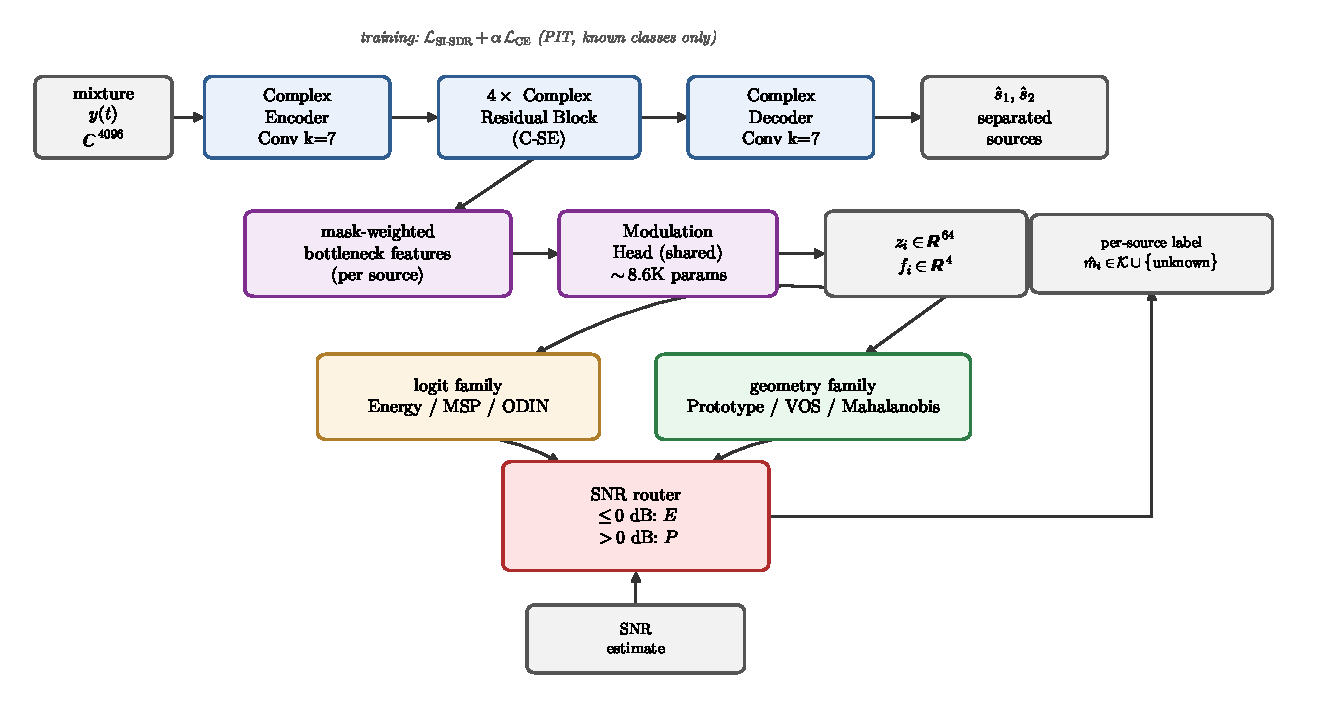
\includegraphics[width=\columnwidth]{figures/fig_architecture.pdf}
\caption{The OpenSetCSE system under study. Top: the C-SE separation
backbone. Bottom: the shared per-source modulation head produces an
embedding $z_i$ and logits $f_i$; the dashed SNR router (Energy at
$\snr \leq \SI{0}{dB}$, Prototype otherwise) is the a-priori routing
rule whose apparent effectiveness was manufactured by the labeling
pitfall of Section~\ref{sec:pitfall} and is re-evaluated under the
corrected protocol of Section~\ref{sec:protocol}.}
\label{fig:arch}
\end{figure}

The separation backbone is a lightweight complex-valued CNN with
complex squeeze-and-excitation (C-SE) channel attention: a complex
encoder (ComplexConv1d + complex batch normalisation), a stack of four
complex residual blocks with C-SE, and a complex decoder producing two
separated waveforms $\hat{s}_1, \hat{s}_2 \in \mathbb{C}^{T}$. On top of the backbone, a
shared per-source \emph{modulation head} aggregates each output's
mask-weighted bottleneck features into a 64-dimensional embedding $z_i$
and $K=4$ logits $f_i$ (one per known modulation). The head adds
$\sim$8.6K parameters; the full model has $\sim$69K parameters.
Training is end-to-end with a permutation-invariant multi-task loss,
\begin{equation}
  \mathcal{L} = \mathcal{L}_{\text{SI-SDR}} + \alpha\,\mathcal{L}_{\text{CE}},
  \label{eq:loss}
\end{equation}
where $\mathcal{L}_{\text{SI-SDR}}$ is the scale-invariant
signal-to-distortion ratio (SI-SDR) loss under the PIT
convention~\cite{kolbaek2017pit,leroux2019sdr} and
$\mathcal{L}_{\text{CE}}$ is the cross-entropy of the per-source
modulation labels under the same permutation; we use $\alpha = 1$.
Only the four known modulations appear in training---no unknown-class
data, synthetic or real, is used at any stage.

\subsection{Per-source OOD scoring}
\label{sec:scorers}

Given per-source embeddings $z \in \mathbb{R}^{64}$ and logits
$f \in \mathbb{R}^{K}$, we evaluate six inference-time scorers (larger
= more OOD):
\begin{align}
  \text{Energy:}\quad
    E(f) &= -\log\textstyle\sum_k \exp f_k, \label{eq:energy}\\
  \text{Prototype:}\quad
    P(z) &= \min_k \| z - \mu_k \|_2, \label{eq:proto}\\
  \text{VOS-inspired:}\quad
    V(z) &= \min_j \| z - v_j \|_2, \label{eq:vos}\\
  \text{Mahalanobis:}\quad
    M(z) &= \min_k (z - \mu_k)^{\top} \Sigma^{-1} (z - \mu_k),
    \label{eq:maha}\\
  \text{MSP:}\quad
    S(f) &= -\max_k \mathrm{softmax}(f)_k, \label{eq:msp}\\
  \text{ODIN:}\quad
    O(x) &= -\max_k \mathrm{softmax}\!\big(f(\tilde{x}) / T\big)_k,
    \label{eq:odin}
\end{align}
with class prototypes $\mu_k$ (and the shared covariance $\Sigma$) fit
on a known-class reference pool, and virtual outliers $v_j$ synthesised
by extrapolation from the class prototypes in the spirit
of~\cite{du2022vos}. We stress that Eq.~\eqref{eq:vos} is
\emph{VOS-inspired}: a training-free, post-hoc heuristic that borrows
the virtual-outlier construction of VOS but applies no outlier-aware
training loss; it should not be read as the original VOS method.
ODIN~\cite{liang2018odin} uses temperature $T = 1000$ and a
perturbation magnitude $\varepsilon = 5\times10^{-3}$ extended to the
complex mixture as
$\tilde{x} = x + \varepsilon\,(\mathrm{sign}\,\Re g + j\,\mathrm{sign}\,\Im g)$,
$g = \nabla_x \log\,\mathrm{softmax}(f/T)_{\hat{y}}$. Since no
unknown-class data is available at validation time by construction,
$\varepsilon$ is fixed a priori rather than tuned. Under the corrected
protocol (Section~\ref{sec:protocol}) the reference statistics
$(\mu_k, \Sigma, v_j)$ are fit on a \emph{disjoint} reference pool
(seed 88888), never on test data.

% ======================================================================
\section{The Pitfall: Repeat-vs-Tile Per-Source SNR Labels}
\label{sec:pitfall}

\subsection{Mechanism}

The evaluation pipeline dumps, for every test sample, per-source OOD
scores and the per-source SNR labels used to bin them. Two different
flattening conventions met at this interface. The per-source score,
embedding, and modulation-label arrays were stacked \emph{tile-wise}:
all slot-1 entries for every mixture, then all slot-2 entries,
\begin{equation}
  \texttt{scores} = \texttt{concatenate}\big([\text{slot 1 of all mixtures},\ \text{slot 2 of all mixtures}]\big),
  \label{eq:tile}
\end{equation}
while the per-source SNR labels were written \emph{interleaved}
(\texttt{np.repeat}): each mixture's SNR twice in a row,
\begin{equation}
  \texttt{snr\_label} = \texttt{np.repeat}(\snr_{\text{mixture}}, 2).
  \label{eq:repeat}
\end{equation}
Entry $j$ of the score array is the $(j \bmod N)$-th mixture's slot
$\lfloor j/N \rfloor + 1$ (true SNR $\snr_{j \bmod N}$), but it was
paired with label $\snr_{\lfloor j/2 \rfloor}$. Because the test set is
generated in SNR blocks (192 mixtures per SNR per protocol), the
misalignment is not random but \emph{structured}: stored ``bin $i$'' of
the known pool in fact contains scores from true bins $2i$ and $2i{+}1$,
and---past the slot-1/slot-2 boundary---from true bins whose SNR differs
from the stored label by up to \SI{15}{dB}
(Fig.~\ref{fig:mechanism}). The unknown pool, whose SNR array was
masked with the same permutation-invariant-training swap masks as its
scores, was always exact. Every ``per-SNR'' AUROC of the known pool
therefore compared known sources at one set of true SNRs against
unknown sources at \emph{another}.

\begin{figure}[H]
\centering
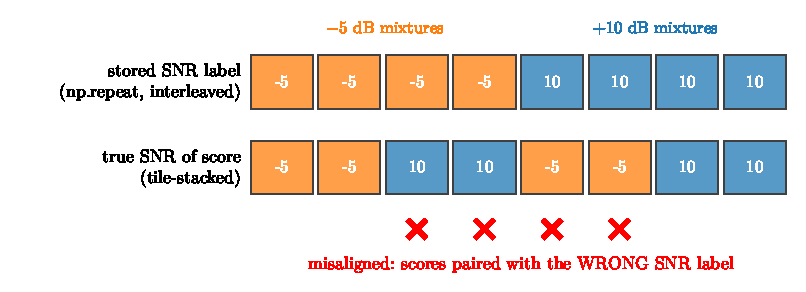
\includegraphics[width=0.85\columnwidth]{figures/fig_pitfall_mechanism.pdf}
\caption{Repeat-vs-tile misalignment on a four-mixture toy example.
The score array is stacked slot-wise (all slot-1, then all slot-2),
so the true SNR sequence of its entries is $[-5, -5, 10, 10, -5, -5,
10, 10]$; the stored label sequence repeats each mixture's SNR
in place, $[-5, -5, -5, -5, 10, 10, 10, 10]$. Half of all entries
(red crosses) are paired with the wrong SNR. In the real test set
(1344 kk mixtures in seven SNR blocks) the same mechanism assigns
every stored ``SNR bin'' of the known pool scores from other true
bins, with label--truth mismatches of up to \SI{15}{dB}.}
\label{fig:mechanism}
\end{figure}

A one-line check exposes the corruption. Binning the stored
\emph{modulation} labels of the known pool by the stored (repeat) SNR
labels gives per-bin class counts $114/96/100/74$---impossible, since
the kk protocol contributes exactly $96$ mixtures of each known
modulation per true SNR bin; binning by the corrected (tile) labels
recovers exactly $96/96/96/96$.

\subsection{The manufactured phenomenon}

Why does the misalignment produce \emph{structure} rather than mere
noise? All OOD score scales drift with SNR: noise flattens logits and
inflates embedding distances. A stored ``bin'' whose known entries
actually come from \emph{lower}-SNR blocks therefore contains known
scores shifted toward the unknown end of the scale (and vice versa),
so the per-bin AUROC measures the score's \emph{SNR separability}
between the mismatched pools---a large, deterministic signal. Because
the Energy score and the Prototype score drift with SNR in opposite
directions relative to the pool imbalance at each stored bin, the
artifact presented as a perfect complementarity: Prototype/VOS-inspired
apparently reached $0.84 \pm 0.02$ AUROC at \SI{10}{dB} while
collapsing below \SI{0}{dB}, and Energy apparently peaked at
$0.74 \pm 0.03$ at \SI{-5}{dB} while falling to $0.22$ at \SI{10}{dB}
(Fig.~\ref{fig:artifact}a). The obvious exploitation---route each
sample to the scorer that ``works'' at its SNR---then appeared to lift
the pair-weighted average AUROC from $0.50$ (pooled) to
$0.625 \pm 0.031$ over five seeds, against a post-hoc oracle bound of
$0.641$ (three scorers) to $0.681$ (six scorers).

The artifact did not stop at the headline. It produced a complete,
internally consistent research narrative, every row of which dissolved
under corrected labels (Table~\ref{tab:artifact}):
simulated SNR-estimation noise of $\sigma = 1/3/6$ dB appeared to
degrade the routed AUROC ``gracefully'' ($0.597/0.593/0.576$);
SIR, timing-offset, and carrier-offset perturbations left it
``robust'' ($0.58$--$0.66$); carrier gaps of 10--\SI{500}{Hz} left it
``unchanged'' ($0.615$--$0.633$); a center-loss intervention appeared to
\emph{hurt} in an informative way ($0.568$); and an embedding-dimension
ablation appeared to show capacity independence ($0.588$--$0.631$).

\begin{table}[H]
\centering
\caption{The artifact catalogue: apparent results produced by the
repeat-vs-tile misalignment vs.\ the same quantities recomputed under
corrected labels (weighted-average per-SNR AUROC, 5 seeds unless
noted). Full corrected numbers in Section~\ref{sec:results}.}
\label{tab:artifact}
{\small
\begin{tabular}{lcc}
\toprule
Quantity & Artifact & Corrected \\
\midrule
SNR-routed ensemble & $0.625 \pm 0.031$ & $0.498 \pm 0.020$ \\
Oracle, 3 scorers (post-hoc) & $0.641$ & $0.514 \pm 0.013$ \\
Oracle, 6 scorers (post-hoc) & $0.681$ & $0.549 \pm 0.031$ \\
SNR noise $\sigma=1/3/6$ dB & $0.597/0.593/0.576$ & $0.502/0.502/0.501$ \\
SIR/timing/CFO (3 seeds) & $0.58$--$0.66$ & $0.487$--$0.494$ \\
Carrier gap 10--\SI{500}{Hz} & $0.615$--$0.633$ & $0.496$--$0.503$ \\
Center loss ($\lambda{=}0.1$) & $0.568$ & $0.487 \pm 0.012$ \\
Embedding dim 16/32/128 (3 seeds) & $0.631/0.588/0.618$ & $0.508/0.477/0.500$ \\
\bottomrule
\end{tabular}}
\end{table}

\begin{figure}[H]
\centering
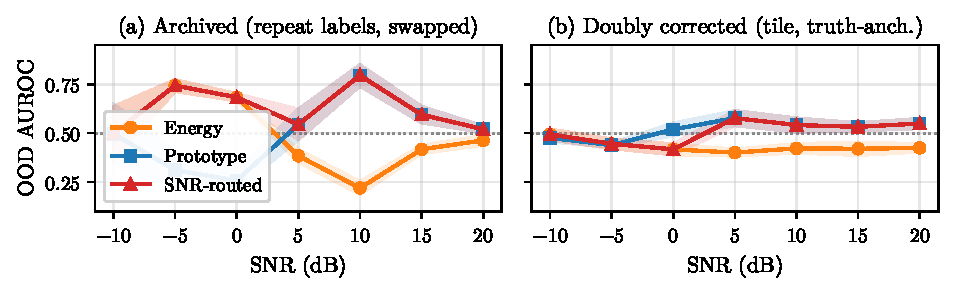
\includegraphics[width=\columnwidth]{figures/fig_artifact_vs_corrected.pdf}
\caption{Per-SNR OOD AUROC of the \emph{same} score dumps (5-seed
mean $\pm$ std) under (a) the buggy repeat labels and (b) the
corrected tile labels. Panel (a) shows the manufactured
complementarity---Energy apparently peaking at low SNR, Prototype at
high SNR, the routed rule apparently following the better branch.
Panel (b) shows the same scores with verified labels: flat at chance
at every SNR\@.}
\label{fig:artifact}
\end{figure}

\subsection{Why the artifact is seductive}

Three properties make this failure mode dangerous, and we list them
because each corresponds to a safeguard that practitioners (including
us) trusted:

\emph{It is systematic, not random.} The misalignment is a deterministic
function of the data layout, identical for every seed, every model,
every condition. Multi-seed averaging therefore does not dilute it---it
\emph{confirms} it, with a comfortably small standard deviation
($\pm 0.031$). Statistical significance testing offers no protection
either: a $p$-value computed on the mislabeled bins is significant
precisely because the SNR-mismatch signal is real; what is wrong is
the interpretation of the bins.

\emph{It survives every robustness check.} SIR imbalance, timing
offsets, and carrier-frequency offsets perturb the signals, not the
label geometry, so the artifact passes the exact perturbation battery
reviewers ask for---and each pass reads as independent evidence. The
simulated SNR-noise sweep is worse: ``graceful degradation'' under
increasing $\sigma$ is precisely what the \emph{artifact} predicts,
because noising the SNR only blurs the SNR-mismatch signal the bins
measure. The check most discriminating between truth and artifact
would have been the one nobody thinks to run: verifying that the
labels themselves are aligned.

\emph{It is mechanistically narratable.} Each artifact number admitted
a plausible post-hoc story (logit-based confidence ``naturally''
inverting at high SNR; geometry-based scores ``naturally'' requiring
de-noised embeddings), which is how the artifact survived internal
scrutiny across two manuscript revisions. A sufficiently flexible
intuition can explain any deterministic pattern; the lesson is that a
convincing mechanism story is not evidence of a correct pipeline.

\subsection{How it was caught}

The bug was not found by a statistical test but by an engineering
necessity. Replacing the oracle SNR in the router with a \emph{real
blind SNR estimator} (Section~\ref{sec:snrest}) required estimating the
SNR from each regenerated test waveform and pairing the estimate with
the stored score of the same sample. The sample-level alignment
verification written for that purpose---regenerate the test set with
its deterministic seed, then check the stored arrays against the data
order element by element---failed immediately: the stored per-source
SNR sequence matched \texttt{np.repeat} while the score array order
matched \texttt{np.tile}. Recomputing every per-SNR quantity under
corrected labels collapsed the routed AUROC to $0.498$. We regard the
verification step itself---\emph{align labels against regenerated data
before trusting any conditioned metric}---as the portable lesson, and
it is now part of the protocol in Section~\ref{sec:protocol}.

% ======================================================================
\section{Corrected, Deployment-Faithful Evaluation Protocol}
\label{sec:protocol}

The corrected protocol changes \emph{how things are measured}, not what
is trained. Its five rules:

\textbf{P1. Verified label alignment.} After any dump, per-source label
arrays are verified against regenerated data: sequence equality of the
per-mixture SNR order, pool sizes, per-bin sample counts, and per-bin
modulation-label multisets (the $96/96/96/96$ check of
Section~\ref{sec:pitfall}). Every number in Section~\ref{sec:results}
comes from dumps that pass all checks on all five seeds.

\textbf{P2. Strict train/reference/test separation.} Training uses its
own stream; OOD reference statistics ($\mu_k, \Sigma, v_j$) are fit on
a \emph{disjoint reference pool} (deterministic seed 88888) drawn under
the test protocol; the test set uses seed 99999. No test sample enters
any fitted quantity. (The artifact-era pipeline had already verified
that re-fitting reference statistics on a held-out pool changed every
AUROC by $<0.003$; the corrected protocol makes the separation
mandatory rather than optional.)

\textbf{P3. Unknown-free threshold calibration.} AUROC is
threshold-free and can hide an unusable operating point. We therefore
also fix a \emph{single global rejection threshold} $\tau$ at the 95th
percentile of the routed score on the reference-pool knowns (a 5\%
false-rejection-rate target), calibrated \emph{without} any
unknown-class data, and report the operational metrics:
Det@$\tau$ (unknown detection rate at $\tau$), FRR@$\tau$,
FPR95, OSCR~\cite{dhamija2018oscr}, and joint accuracy (known accepted
and correctly classified, plus unknown rejected, over all samples).
Because Energy and Prototype scores live on disjoint scales, the
routed score is calibrated on the reference pool directly, with
routed low-SNR reference samples handled by a provable below-threshold
argument (score ranges verified per seed).

\textbf{P4. A-priori routing decisions.} The routing boundary
(\SI{0}{dB}) is fixed a priori from training-range profiles, never
tuned on test data; the post-hoc per-bin oracle is reported separately
and interpreted as an upper bound subject to max-selection bias, not
as an achievable number.

\textbf{P5. Real blind SNR estimation for deployed routing.} A deployed
router cannot read the true SNR\@. We use a validated blind subspace
estimator (Section~\ref{sec:snrest}) and report routing both with the
estimate and, for diagnosis, with ground truth.

\subsection{A validated blind SNR estimator}
\label{sec:snrest}

The estimator is waveform-only: the noise floor is read off as the
median eigenvalue of the $L{=}64$ Toeplitz autocorrelation matrix of
the received mixture, and the signal power follows by subtraction.
Table~\ref{tab:snrest} summarises its quality on all 3360 test
mixtures (480 per SNR bin): per-bin bias between $-0.57$ and
$-0.61$ dB at the extremes and within $-0.24$ dB mid-range, overall
RMSE \SI{0.51}{dB} (bias $-0.31$ dB, std $0.40$ dB), uniformly across
kk/ku/uu protocols (per-protocol RMSE within $0.17$--$0.92$ dB per
bin). The classical M2M4 moment estimator~\cite{pauluzzi2000snr} is
inadequate for this signal class (overall RMSE \SI{13.99}{dB}): its
kurtosis assumption breaks for two-source co-frequency mixtures with
RRC pulse shaping and three-tap multipath---the mixture's measured
fourth moment is dominated by the cross-term of the two sources and by
the channel-induced constellation spread rather than by the
single-source modulation kurtosis the estimator is calibrated on, so
its SNR read-out saturates and compresses
(Fig.~\ref{fig:snrest}). Equivalent Gaussian-noise calibration places
the subspace estimator at $\sigma \approx \SI{0.51}{dB}$.

\begin{table}[H]
\centering
\caption{Blind SNR-estimation quality (all 3360 test mixtures, 480 per
bin). Subspace = median-eigenvalue of the Toeplitz autocorrelation;
M2M4 shown for contrast.}
\label{tab:snrest}
{\small
\begin{tabular}{lccc}
\toprule
True SNR (dB) & Bias (dB) & Std (dB) & RMSE (dB) \\
\midrule
$-10$ & $-0.57$ & $0.59$ & $0.82$ \\
$-5$  & $-0.24$ & $0.26$ & $0.35$ \\
$0$   & $-0.14$ & $0.15$ & $0.20$ \\
$+5$  & $-0.14$ & $0.12$ & $0.18$ \\
$+10$ & $-0.17$ & $0.17$ & $0.24$ \\
$+15$ & $-0.30$ & $0.22$ & $0.37$ \\
$+20$ & $-0.61$ & $0.59$ & $0.85$ \\
\midrule
Overall & $-0.31$ & $0.40$ & $0.51$ \\
M2M4 overall & $-8.71$ & $10.95$ & $13.99$ \\
\bottomrule
\end{tabular}}
\end{table}

\begin{figure}[H]
\centering
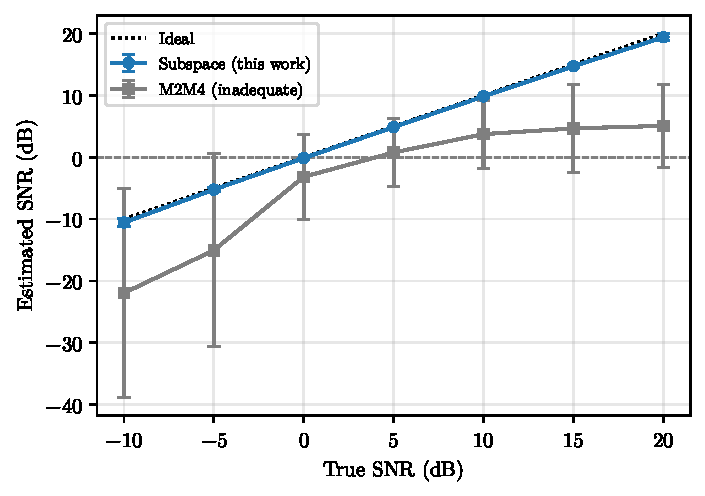
\includegraphics[width=0.6\columnwidth]{figures/fig_snr_estimator.pdf}
\caption{True vs.\ estimated SNR (mean $\pm$ std over 480 mixtures per
bin). The subspace estimator tracks the ideal line across the full
$[-10, 20]$ dB range; M2M4 saturates and is unusable for this signal
class.}
\label{fig:snrest}
\end{figure}

% ======================================================================
\section{Corrected Results: A Systematic Negative Result}
\label{sec:results}

\subsection{Setup}
\label{sec:expsetup}

\emph{Data.} All signals are synthetic complex baseband waveforms:
linear modulations (and OFDM-QPSK) with root-raised-cosine pulse
shaping, a three-tap multipath fading channel, and additive white
Gaussian noise~\cite{proakis2008digital}. Each mixture contains two
sources with carrier frequencies \SI{2000}{Hz} and \SI{2005}{Hz}
(each with an independent $\pm$\SI{5}{Hz} jitter) at
$T = 4096$ samples and a \SI{16}{kHz} sample rate. Training SNR is
uniform in $[-5, 20]$ dB; test SNR spans
$\{-10, -5, 0, 5, 10, 15, 20\}$ dB, i.e.\ including SNRs \emph{below}
the training range. Test sets are deterministic (seed 99999) with 200
mixtures per SNR for the kk/ku protocols and 100 for uu; the reference
pool uses seed 88888. No external dataset is required; the generator is
released with the code.

\emph{Training.} OpenSetCSE ($\sim$69K parameters), 100 epochs, batch
size 16, Adam at $10^{-3}$, loss of Eq.~\eqref{eq:loss} with
$\alpha = 1$. Five seeds (42--46).
\emph{Every} reported number is multi-seed---necessary, though this
paper demonstrates at some length that it is not \emph{sufficient}.

\subsection{Closed-set sanity}
\label{sec:closed}

Table~\ref{tab:closed} shows that the backbone itself works and is
unaffected by the pitfall (the closed-set path builds its masks
consistently): SI-SDR turns positive at $\snr \geq \SI{10}{dB}$ and
closed-set classification accuracy is $0.41$ (chance $0.25$). The
difficulty addressed in this paper is genuinely in OOD detection, not
separation. Pooled (all-SNR) OOD AUROCs are likewise unaffected by the
pitfall---they use no SNR labels---and were honest all along
(Table~\ref{tab:pooled}).

\begin{table}[H]
\centering
\caption{Closed-set (kk) performance, 5-seed mean $\pm$ std (unaffected
by the pitfall).}
\label{tab:closed}
\begin{tabular}{lc}
\toprule
Metric & Value \\
\midrule
Pooled SI-SDR (dB) & $-0.88 \pm 0.09$ \\
SI-SDR at \SI{10}{dB} (dB) & $+0.47 \pm 0.14$ \\
SI-SDR at \SI{20}{dB} (dB) & $+0.67 \pm 0.16$ \\
Classification accuracy & $0.407 \pm 0.030$ \\
\bottomrule
\end{tabular}
\end{table}

\begin{table}[H]
\centering
\caption{Pooled OOD AUROC (all SNRs mixed), 5-seed mean $\pm$ std
(unaffected by the pitfall). All scorers are near chance.}
\label{tab:pooled}
\begin{tabular}{lc}
\toprule
Scorer & Pooled AUROC \\
\midrule
Energy      & $0.482 \pm 0.018$ \\
Prototype   & $0.509 \pm 0.013$ \\
VOS-inspired & $0.509 \pm 0.013$ \\
Mahalanobis & $0.524 \pm 0.046$ \\
MSP         & $0.433 \pm 0.010$ \\
ODIN        & $0.486 \pm 0.016$ \\
\bottomrule
\end{tabular}
\end{table}

\subsection{Corrected per-SNR profiles: flat everywhere}
\label{sec:flat}

Fig.~\ref{fig:artifact}b already showed the corrected Energy/Prototype
profiles; Fig.~\ref{fig:all6} extends this to all six scorers. Every
scorer sits within seed noise of chance at every SNR (per-bin range
roughly $0.42$--$0.60$, all within $\sim$2 standard errors of $0.5$);
no scorer family works at any SNR, and there is no complementarity
left to exploit. Table~\ref{tab:main} quantifies the summary: the
a-priori SNR-routed ensemble reaches $0.498 \pm 0.020$---exactly
chance. The post-hoc oracle over the three primary scorers is
$0.514 \pm 0.013$, and over all six scorers $0.549 \pm 0.031$. The
six-scorer oracle deserves a caveat: it takes a per-bin \emph{maximum}
over six scorers after seeing the data, so it is biased above $0.5$ by
construction (max-selection on seven bins), and even so it reaches
only $0.55$. The deployable, a-priori quantities---single scorers and
the routed rule---are at chance. Mahalanobis, the strongest single
scorer ($0.521 \pm 0.050$ weighted, $0.524 \pm 0.046$ pooled), owes its
margin largely to one seed and stays within seed noise of chance.

\begin{table}[H]
\centering
\caption{Corrected main result: weighted-average per-SNR AUROC, 5-seed
mean $\pm$ std (pair-weighted bins, verified labels). Oracle =
post-hoc best scorer per bin (upper bound, max-selection biased).}
\label{tab:main}
\begin{tabular}{lc}
\toprule
Scorer & Weighted-avg AUROC \\
\midrule
Energy      & $0.476 \pm 0.019$ \\
Prototype   & $0.506 \pm 0.010$ \\
VOS-inspired & $0.505 \pm 0.010$ \\
Mahalanobis & $0.521 \pm 0.050$ \\
MSP         & $0.431 \pm 0.009$ \\
ODIN        & $0.480 \pm 0.019$ \\
\midrule
SNR-routed (a-priori rule) & $0.498 \pm 0.020$ \\
Oracle, 3 scorers (post-hoc) & $0.514 \pm 0.013$ \\
Oracle, 6 scorers (post-hoc) & $0.549 \pm 0.031$ \\
\bottomrule
\end{tabular}
\end{table}

\begin{figure}[H]
\centering
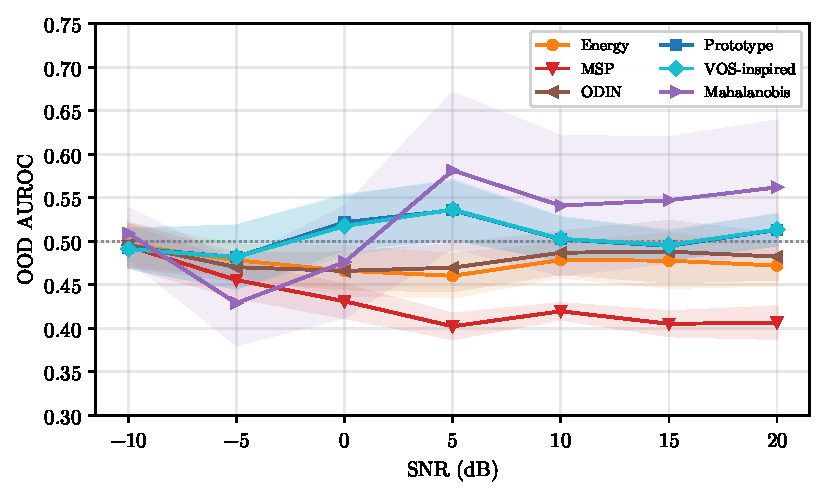
\includegraphics[width=0.7\columnwidth]{figures/fig_per_snr_all6.pdf}
\caption{Corrected per-SNR OOD AUROC of all six scorers (5-seed mean
$\pm$ std). Every profile is flat at chance; the artifact's apparent
complementarity (Fig.~\ref{fig:artifact}a) is gone.}
\label{fig:all6}
\end{figure}

\subsection{Robustness: flat under every perturbation}
\label{sec:robust}

The artifact's robustness narrative inverts: under corrected labels
there is nothing left to degrade. Simulated SNR-estimation noise of
$\sigma = 1/3/6$ dB leaves the routed AUROC at
$0.502/0.502/0.501$ ($\pm 0.014$--$0.018$; 50 Monte-Carlo trials per
seed)---flat, because there is no routing gain to lose. The same holds
under the physical perturbations of Table~\ref{tab:robust}: SIR from
$-6$ to $+6$ dB, random symbol-timing offsets, and a \SI{25}{Hz}
carrier jitter all leave the routed AUROC within $0.487$--$0.494$
(3 seeds). Routing with the \emph{estimated} SNR from the subspace
estimator of Section~\ref{sec:snrest} gives $0.501 \pm 0.017$ on
corrected true-SNR bins (fully deployed, estimated-SNR bins:
$0.471 \pm 0.014$; M2M4: $0.444$)---again chance, confirming that the
estimator quality is no longer a bottleneck because there is no gain
for it to bottleneck.

\begin{table}[H]
\centering
\caption{Corrected routed weighted-avg AUROC under channel
perturbations (3 seeds, mean $\pm$ std; ground-truth SNR routing,
a-priori \SI{0}{dB} boundary).}
\label{tab:robust}
\begin{tabular}{lc}
\toprule
Condition & Routed AUROC \\
\midrule
Baseline & $0.487 \pm 0.014$ \\
SIR $-6$ dB & $0.494 \pm 0.008$ \\
SIR $-3$ dB & $0.490 \pm 0.007$ \\
SIR $0$ dB & $0.490 \pm 0.012$ \\
SIR $+3$ dB & $0.490 \pm 0.011$ \\
SIR $+6$ dB & $0.492 \pm 0.009$ \\
Timing offset & $0.492 \pm 0.009$ \\
CFO jitter \SI{25}{Hz} & $0.490 \pm 0.011$ \\
\bottomrule
\end{tabular}
\end{table}

\subsection{Interventions: training side, capacity, carrier gap}
\label{sec:interventions}

\emph{Center loss} ($\lambda{=}0.1$, 5 seeds)~\cite{wen2016center}:
routed $0.487 \pm 0.012$, oracle $0.502 \pm 0.009$---no gain. The
artifact-era reading (``center loss weakens the high-SNR prototype
signal the router relies on'') was a story about a signal that did not
exist; the corrected reading is simpler: within-class compactness
shaping cannot create a margin against classes never seen in training.

\emph{Embedding dimension} (16/32/64/128, 3 seeds): routed
$0.508$, $0.477$, $0.498$, $0.500$; oracles
$0.530$, $0.505$, $0.514$, $0.517$---flat and
non-monotone. OOD performance is not capacity-limited.

\emph{Carrier-frequency separation} (10/50/100/\SI{500}{Hz}, model
trained at \SI{5}{Hz}, 5 seeds): routed
$0.500 \pm 0.022 / 0.503 \pm 0.020 / 0.496 \pm 0.018 / 0.503 \pm 0.011$.
The negative result is not an artifact of the training carrier gap.

\subsection{Single-threshold operating point}
\label{sec:oppoint}

AUROC can hide an unusable operating point; the deployment question is
what happens at one calibrated threshold. Under protocol rule P3
(reference-pool calibration, 5\% FRR target, no unknown-class data),
Table~\ref{tab:oppoint} and Fig.~\ref{fig:oppoint} give the operational
truth: the routed detector rejects only $0.058 \pm 0.038$ of unknown
sources at its calibrated threshold, with OSCR $0.197 \pm 0.012$ and
joint known/unknown accuracy $0.217 \pm 0.028$. The per-SNR breakdown
shows the detection rate is \emph{exactly zero} at and below
\SI{0}{dB} and reaches only $0.15$ even at \SI{20}{dB}: at a single,
honestly calibrated operating point, the system detects essentially no
unknown sources anywhere. A rank-normalised variant (each scorer mapped
through its known-pool empirical CDF before routing, so a single
threshold is scale-fair) changes the picture only marginally (Det
$0.070 \pm 0.031$).

\begin{table}[H]
\centering
\caption{Single-threshold operating point (protocol rule P3; threshold
$\tau$ = 95th percentile of reference-pool known scores, 5\% FRR
target; 5 seeds, mean $\pm$ std). Det@$\tau$ = unknown detection rate.}
\label{tab:oppoint}
{\footnotesize\setlength{\tabcolsep}{3pt}
\begin{tabular}{lccccc}
\toprule
Method & Det@$\tau$ & FRR@$\tau$ & FPR95 & OSCR & JointAcc \\
\midrule
Routed & $0.058 \pm 0.038$ & $0.051 \pm 0.003$ & $0.954 \pm 0.010$ & $0.197 \pm 0.012$ & $0.217 \pm 0.028$ \\
Prototype & $0.058 \pm 0.038$ & $0.051 \pm 0.003$ & $0.947 \pm 0.013$ & $0.190 \pm 0.013$ & $0.217 \pm 0.028$ \\
VOS-inspired & $0.058 \pm 0.037$ & $0.051 \pm 0.003$ & $0.947 \pm 0.012$ & $0.190 \pm 0.012$ & $0.217 \pm 0.027$ \\
\bottomrule
\end{tabular}}
\end{table}

\begin{figure}[H]
\centering
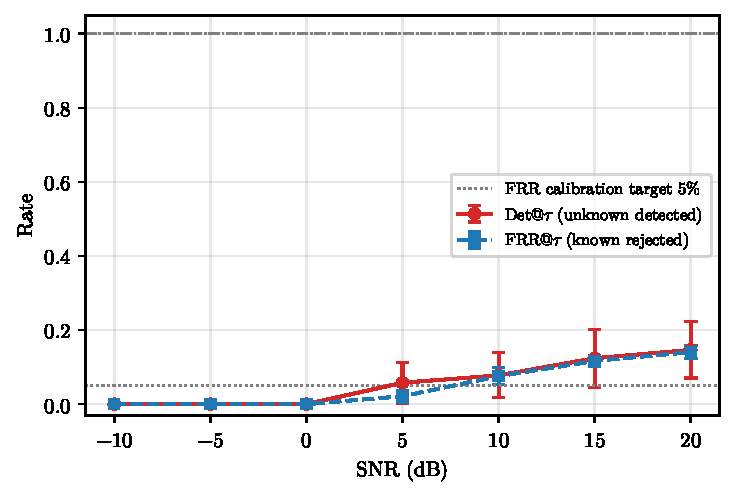
\includegraphics[width=0.6\columnwidth]{figures/fig_operating_point.pdf}
\caption{Per-SNR operating point of the routed detector at the
calibrated threshold (variant of Table~\ref{tab:oppoint}): unknown
detection rate Det@$\tau$ and known false-rejection rate FRR@$\tau$.
Detection is exactly $0$ at $\snr \leq \SI{0}{dB}$ and reaches only
$0.15$ at \SI{20}{dB}---the detector is operationally blind to unknown
sources at a 5\% FRR budget.}
\label{fig:oppoint}
\end{figure}

\subsection{Leave-one-modulation-out and cross-backbone checks}
\label{sec:lomo}

\emph{Leave-one-modulation-out (LOMO).} Each known modulation in turn is
held out of training (3-mod known alphabet) and added to the unknown
pool at test time; the routing boundary is selected on a pseudo-OOD
\emph{validation} split (seed 77777, the held-out known class playing
the unknown role---never touching test data), i.e.\ the boundary is
chosen \emph{legally}, with no test unknowns and no oracle SNR
profiling. Table~\ref{tab:lomo} gives the full $4 \times 3$ grid. Two
observations, both consistent with the rest of this paper. First, the
legally selected boundary is \emph{unstable}: 9 of 12 runs select
\SI{0}{dB}, but 3 of 12 find no usable crossover and fall back to an
all-Prototype route (\SI{20}{dB})---unstable precisely because, per
Section~\ref{sec:flat}, there is no real crossover to find. Second, the
routed AUROC stays at chance ($0.468$--$0.516$) in every split and
every seed, matching the corrected baseline $0.498$; holding out one
known modulation at a time does not create detectability either.

\begin{table}[H]
\centering
\caption{LOMO: routed weighted-avg AUROC (test seed 99999; unknown pool
= held-out known modulation + the four real unknowns; routing boundary
selected on pseudo-OOD validation seed 77777 only). ``Boundary'' is the
validation-selected SNR switch; \SI{20}{dB} = no crossover found, an
all-Prototype route.}
\label{tab:lomo}
\begin{tabular}{lcccc}
\toprule
Held-out & Seed 42 & Seed 43 & Seed 44 & Mean $\pm$ std \\
\midrule
QPSK  & \SI{0}{dB}, $0.516$ & \SI{0}{dB}, $0.505$ & \SI{20}{dB}, $0.501$ & $0.508 \pm 0.008$ \\
8PSK  & \SI{0}{dB}, $0.514$ & \SI{0}{dB}, $0.506$ & \SI{20}{dB}, $0.506$ & $0.509 \pm 0.005$ \\
16QAM & \SI{0}{dB}, $0.481$ & \SI{0}{dB}, $0.493$ & \SI{0}{dB}, $0.472$  & $0.482 \pm 0.011$ \\
BPSK  & \SI{0}{dB}, $0.498$ & \SI{0}{dB}, $0.468$ & \SI{20}{dB}, $0.491$ & $0.486 \pm 0.016$ \\
\bottomrule
\end{tabular}
\end{table}

\emph{Cross-backbone (no-SE ablation).} To check whether the negative
result is specific to the C-SE backbone, we repeated the full pipeline
with the SE blocks removed (\texttt{--no\_se}, 3 seeds, 60.8K
parameters). The no-SE variant is a strictly weaker separator (pooled
SI-SDR $-1.15$~dB vs.\ $-0.88$~dB; closed-set accuracy $0.356$ vs.\
$0.407$), yet the corrected evaluation looks the same: routed
weighted-avg AUROC $0.508 \pm 0.011$, single scorers $0.491 \pm 0.031$
(Energy), $0.531 \pm 0.012$ (Prototype), $0.532 \pm 0.011$
(VOS-inspired), and a three-scorer oracle of $0.536 \pm 0.014$.
Prototype sits marginally above chance ($\approx 0.53$), but its
per-SNR profile shows no low/high-SNR complementarity with Energy
(Energy is flat at $0.47$--$0.50$ across SNR), so there is again
nothing for a router to exploit. The scorer-inversion phenomenon
appears in \emph{neither} backbone once the labels are correct: it was
a property of the mislabeled evaluation, not of any feature
representation.

% ======================================================================
\section{Discussion: Attribution and Lessons}
\label{sec:disc}

\subsection{Why is detection at chance?}

The negative result is over-determined by the controls, and the
attribution points at the training objective rather than the readout.

\emph{The objective shapes no known/unknown margin.}
Eq.~\eqref{eq:loss} asks the network to (i) reconstruct waveforms
permutation-invariantly and (ii) classify the four known modulations.
Nothing in it references out-of-alphabet signals: the network is never
shown one, never penalised for mapping one close to a known prototype,
and---because waveform reconstruction at this difficulty level is
largely modulation-agnostic (RRC pulses through a three-tap channel
carrying 2--16 point constellations)---never even pressured to encode
modulation beyond what the four-way head needs. The unknown
modulations are moreover \emph{same-family neighbours} of the known
ones (64QAM vs.\ 16QAM; $\pi$/4-DQPSK vs.\ PSKs; MSK vs.\ BPSK-like
CPM), so their embeddings land inside the known support at every SNR.

\emph{The controls exclude the alternatives.} If the failure were
readout capacity, widening the embedding would help---it does not
($0.477$--$0.508$ over $16$--$128$ dims). If it were within-class
scatter, center loss would help---it does not ($0.487$). If it were a
property of one scorer family, some member of the six would separate
somewhere---none does, and the post-hoc ceiling over all six is
$0.549$, max-selection bias included. If it were the carrier
separation or channel conditions, the gap/perturbation sweeps would
move it---they do not. The remaining explanation is the simplest: the
features contain no usable known/unknown signal to begin with.

\emph{Consequence for practice.} An open-set SC-BSS receiver cannot
expect post-hoc OOD scoring of separation embeddings to flag unknown
modulations; the capability, if wanted, must be \emph{built in} at
training time (outlier exposure, margin-shaping losses, explicit
abstention heads) or sourced from modulation-specific signal structure
rather than generic embeddings. Whether such training-side mechanisms
help on this benchmark is an open question the corrected protocol is
designed to answer honestly.

\subsection{A protocol checklist for conditioned OOD evaluation}

We distill what would have caught the pitfall early, and what the
corrected study needed. None of these is expensive; all are cheap
relative to a manuscript built on an artifact.

\begin{enumerate}
  \item \textbf{Align labels against regenerated data.} Whenever a
        metric is conditioned on a per-sample variable, regenerate the
        deterministic test set and verify every label array against the
        data order (sequence equality, per-bin counts, per-bin label
        multisets). This single step catches the entire repeat/tile
        family.
  \item \textbf{Be suspicious of flattering structure.} A dramatic,
        mechanistically convenient pattern (scorer rankings inverting
        on cue) warrants pipeline verification \emph{before}
        narrative-building, not after.
  \item \textbf{Multi-seed averaging is not a pipeline check.} It
        averages away random error and confirms systematic error.
        Statistical significance likewise says nothing about label
        correctness.
  \item \textbf{Separate train / reference / test strictly.} Reference
        statistics and thresholds fitted on test data are leakage even
        when their measured influence is small; make the separation
        structural (distinct deterministic seeds), not cosmetic.
  \item \textbf{Calibrate operating points without unknown-class
        data.} Report Det@$\tau$ at an unknown-free threshold alongside
        AUROC; a scorer can look acceptable in AUROC while rejecting
        nothing at any deployable threshold (here: Det $= 0.058$).
  \item \textbf{Treat oracle bounds as bounds.} Per-bin post-hoc maxima
        over $S$ scorers are biased upward by selection; report them
        with the deployable a-priori rule, never as the headline.
  \item \textbf{Use real estimators for operating-condition
        variables.} An oracle-SNR router can hide a large deployment
        gap; validating the estimator (Table~\ref{tab:snrest}) forced
        the alignment check that exposed the pitfall.
\end{enumerate}

% ======================================================================
\section{Limitations}
\label{sec:limit}

The negative result is bounded in scope. Data are synthetic (RRC pulse
shaping, three-tap multipath, AWGN); real-world impairments could move
the picture in either direction. Scenarios are two-source ($K{=}2$) with
symbol-aligned sources and a modest known alphabet. The evidence covers
one separator family (C-SE CNN, $\sim$69K parameters, plus its no-SE
ablation)---and
post-hoc scorers only: training-side open-set mechanisms (outlier
exposure, VOS-style losses on synthetic outliers, abstention heads) are
explicitly out of scope and remain the most plausible way to change
the picture.
Finally, the SNR estimator is validated on the same synthetic signal
class it is used on.

% ======================================================================
\section{Conclusion}
\label{sec:concl}

We set out to evaluate open-set per-source modulation detection on top
of a single-channel blind separator, and found two things. First, a
cautionary one: a one-line repeat-vs-tile mismatch between per-source
SNR labels and per-source score arrays manufactured an entire apparent
phenomenon---SNR-dependent scorer complementarity, a $0.625$ routed
AUROC, graceful degradation, perturbation robustness---that survived
multi-seed averaging, significance intuition, and every robustness
check, and fell only to sample-level label alignment verification.
Second, a clean negative one: under a corrected, deployment-faithful
protocol, post-hoc OOD detection of unknown modulations from
separation embeddings is at chance across six scorers, five seeds,
channel perturbations, training-side and capacity interventions,
carrier separations, leave-one-modulation-out splits, a second
attention-free backbone, and single-threshold operating points, because
the separation objective shapes no known/unknown margin. We release
the corrected pipeline and the archived artifact dumps together, and
hope both the pitfall analysis and the protocol checklist prove useful
to the growing literature on open-set evaluation in signal processing.

% ======================================================================
\section*{CRediT authorship contribution statement}
\textbf{Bin Nong:} Conceptualization, Methodology, Software, Validation,
Formal analysis, Investigation, Data curation, Writing -- original
draft, Visualization.
\textbf{Weihong Fu:} Supervision, Project administration, Writing --
review \& editing.
\textbf{Zhuoyun Jiang:} Resources, Validation, Writing -- review \&
editing.

\section*{Declaration of competing interest}
The authors declare that they have no known competing financial
interests or personal relationships that could have appeared to
influence the work reported in this paper.

\section*{Data availability}
Code, synthetic data generators, the corrected evaluation protocol, and
both the corrected and the archived (artifact-laden) score dumps are
available at
\url{https://github.com/BinNong/single_channel_source_seperation/tree/main/paper3_open_set}.
No external datasets are required.

\section*{Funding}
This research did not receive any specific grant from funding agencies
in the public, commercial, or not-for-profit sectors.

\section*{Declaration of generative AI and AI-assisted technologies in the writing process}
During the preparation of this work the authors used Claude Code
(Anthropic) in order to assist with drafting, editing, and polishing the
manuscript text. After using this tool, the authors reviewed and edited
the content as needed and take full responsibility for the content of
the publication.

% ======================================================================
% Bibliography ordered by first citation (elsarticle numbered style).
\begin{thebibliography}{30}\footnotesize

\bibitem{hou2022single}
X.~Hou and Y.~Gao,
``Single-channel blind separation of co-frequency signals based on
convolutional network,''
\emph{Digital Signal Processing}, vol.~129, p.~103654, 2022,
doi:~\url{https://doi.org/10.1016/j.dsp.2022.103654}.

\bibitem{guo2024single}
P.~Guo, M.~Yu, L.~Shen, Z.~Lin, K.~An, and J.~Wang,
``Single-channel blind source separation in wireless communications: a
complex-domain deep learning approach,''
\emph{IEEE Wireless Commun. Lett.}, vol.~13, no.~6, pp.~1645--1649,
2024, doi:~\url{https://doi.org/10.1109/LWC.2024.3384813}.

\bibitem{hendrycks2017msp}
D.~Hendrycks and K.~Gimpel,
``A baseline for detecting misclassified and out-of-distribution
examples in neural networks,''
in \emph{Proc. ICLR}, 2017.

\bibitem{liang2018odin}
S.~Liang, Y.~Li, and R.~Srikant,
``Enhancing the reliability of out-of-distribution image detection in
neural networks,''
in \emph{Proc. ICLR}, 2018.

\bibitem{liu2020energy}
W.~Liu, X.~Wang, J.~D. Owens, and Y.~Li,
``Energy-based out-of-distribution detection,''
in \emph{Proc. NeurIPS}, 2020.

\bibitem{lee2018mahalanobis}
K.~Lee, K.~Lee, H.~Lee, and J.~Shin,
``A simple unified framework for detecting out-of-distribution samples
and adversarial attacks,''
in \emph{Proc. NeurIPS}, 2018.

\bibitem{du2022vos}
X.~Du, Z.~Wang, M.~Cai, and Y.~Li,
``VOS: Learning what you don't know by virtual outlier synthesis,''
in \emph{Proc. ICLR}, 2022.

\bibitem{proakis2008digital}
J.~G.~Proakis and M.~Salehi,
\emph{Digital Communications}, 5th~ed., McGraw-Hill, 2008.

\bibitem{oshea2017intro}
T.~O'Shea and J.~Hoydis,
``An introduction to deep learning for the physical layer,''
\emph{IEEE Trans. Cogn. Commun. Netw.}, vol.~3, no.~4, pp.~563--575,
2017, doi:~\url{https://doi.org/10.1109/TCCN.2017.2758370}.

\bibitem{dhamija2018oscr}
A.~Dhamija, M.~G{\"u}nther, and T.~Boult,
``Reducing network agnostophobia,''
in \emph{Proc. NeurIPS}, 2018.

\bibitem{hyvarinen2000ica}
A.~Hyv{\"a}rinen and E.~Oja,
``Independent component analysis: algorithms and applications,''
\emph{Neural Netw.}, vol.~13, no.~4--5, pp.~411--430, 2000,
doi:~\url{https://doi.org/10.1016/S0893-6080(00)00026-5}.

\bibitem{chen2019deep}
C.~Chen, Z.~Lu, Z.~Guo, F.~Yang, and L.~Ding,
``Deep learning based single-channel blind separation of co-frequency
modulated signals,''
in \emph{Proc. ChinaCom}, 2019, pp.~607--618,
doi:~\url{https://doi.org/10.1007/978-3-030-41114-5_45}.

\bibitem{ma2023novel}
H.~Ma, X.~Zheng, L.~Yu, et~al.,
``A novel end-to-end deep separation network based on attention
mechanism for single channel blind separation in wireless
communication,''
\emph{IET Signal Process.}, vol.~17, no.~2, p.~e12173, 2023,
doi:~\url{https://doi.org/10.1049/sil2.12173}.

\bibitem{luo2023single}
W.~Luo, R.~Yang, H.~Jin, et~al.,
``Single channel blind source separation of complex signals based on
spatial-temporal fusion deep learning,''
\emph{IET Radar, Sonar Navig.}, vol.~17, no.~2, pp.~200--211, 2023,
doi:~\url{https://doi.org/10.1049/rsn2.12333}.

\bibitem{s4unet2026}
S.~Gao, W.~Guo, H.~Shi, and R.~Peng,
``S4-UNET: a long-sequence modeling blind source separation method for
single-channel co-channel overlapped communication signals,''
\emph{J. Electron. Inf. Technol.}, vol.~48, no.~6, pp.~2384--2395,
2026, doi:~\url{https://doi.org/10.11999/JEIT251144}.

\bibitem{deng2024co}
W.~Deng, X.~Wang, and Z.~Huang,
``Co-channel multiuser modulation classification using data-driven blind
signal separation,''
\emph{IEEE Internet Things J.}, vol.~11, no.~8, pp.~14829--14843, 2024,
doi:~\url{https://doi.org/10.1109/JIOT.2023.3345023}.

\bibitem{trabelsi2018complex}
C.~Trabelsi, O.~Bilaniuk, Y.~Zhang, D.~Serdyuk, S.~Subramanian,
J.~F. Santos, S.~Mehri, N.~Rostamzadeh, Y.~Bengio, and C.~J. Pal,
``Deep complex networks,''
in \emph{Proc. ICLR}, 2018.

\bibitem{lee2022complex}
C.~Lee, H.~Hasegawa, and S.~Gao,
``Complex-valued neural networks: a comprehensive survey,''
\emph{IEEE/CAA J. Autom. Sinica}, vol.~9, no.~8, pp.~1406--1426, 2022,
doi:~\url{https://doi.org/10.1109/JAS.2022.105743}.

\bibitem{hu2018senet}
J.~Hu, L.~Shen, and G.~Sun,
``Squeeze-and-excitation networks,''
in \emph{Proc. CVPR}, 2018, pp.~7132--7141,
doi:~\url{https://doi.org/10.1109/CVPR.2018.00745}.

\bibitem{scheirer2013open}
W.~J. Scheirer, A.~de~Rezende~Rocha, A.~Sapkota, and T.~E. Boult,
``Toward open set recognition,''
\emph{IEEE Trans. Pattern Anal. Mach. Intell.}, vol.~35, no.~7,
pp.~1757--1772, 2013, doi:~\url{https://doi.org/10.1109/TPAMI.2012.256}.

\bibitem{bendale2016openmax}
A.~Bendale and T.~E. Boult,
``Towards open set deep networks,''
in \emph{Proc. CVPR}, 2016, pp.~1563--1572,
doi:~\url{https://doi.org/10.1109/CVPR.2016.173}.

\bibitem{wen2016center}
Y.~Wen, K.~Zhang, Z.~Li, and Y.~Qiao,
``A discriminative feature learning approach for deep face
recognition,''
in \emph{Proc. ECCV}, 2016, pp.~499--515,
doi:~\url{https://doi.org/10.1007/978-3-319-46478-7_31}.

\bibitem{vaze2022open}
S.~Vaze, K.~Han, A.~Vedaldi, and A.~Zisserman,
``Open-set recognition: a good closed-set classifier is all you need?''
in \emph{Proc. ICLR}, 2022.

\bibitem{yang2022openood}
J.~Yang, P.~Wang, D.~Zou, Z.~Zhou, K.~Ding, W.~Peng, H.~Wang,
G.~Chen, B.~Li, Y.~Sun, X.~Du, K.~Zhou, W.~Zhang, D.~Hendrycks, Y.~Li,
and Z.~Liu,
``OpenOOD: Benchmarking generalized out-of-distribution detection,''
in \emph{Proc. NeurIPS (Datasets and Benchmarks)}, 2022.

\bibitem{kapoor2023leakage}
S.~Kapoor and A.~Narayanan,
``Leakage and the reproducibility crisis in machine-learning-based
science,''
\emph{Patterns}, vol.~4, no.~9, p.~100804, 2023,
doi:~\url{https://doi.org/10.1016/j.patter.2023.100804}.

\bibitem{musgrave2020reality}
K.~Musgrave, S.~Belongie, and S.-N. Lim,
``A metric learning reality check,''
in \emph{Proc. ECCV}, 2020, pp.~681--699,
doi:~\url{https://doi.org/10.1007/978-3-030-58595-2_41}.

\bibitem{pauluzzi2000snr}
D.~R.~Pauluzzi and N.~C.~Beaulieu,
``A comparison of SNR estimation techniques for the AWGN channel,''
\emph{IEEE Trans. Commun.}, vol.~48, no.~10, pp.~1681--1691, 2000,
doi:~\url{https://doi.org/10.1109/26.871393}.

\bibitem{kolbaek2017pit}
M.~Kolb{\ae}k, D.~Yu, Z.-H. Tan, and J.~Jensen,
``Multitalker speech separation with utterance-level permutation
invariant training of deep recurrent neural networks,''
\emph{IEEE/ACM Trans. Audio, Speech, Lang. Process.}, vol.~25, no.~10,
pp.~1901--1913, 2017,
doi:~\url{https://doi.org/10.1109/TASLP.2017.2726762}.

\bibitem{leroux2019sdr}
J.~Le~Roux, S.~Wisdom, H.~Erdogan, and J.~R.~Hershey,
``SDR---half-baked or well done?,''
in \emph{Proc. ICASSP}, 2019, pp.~626--630,
doi:~\url{https://doi.org/10.1109/ICASSP.2019.8683855}.

\end{thebibliography}

\end{document}
